\documentclass[journal]{IEEEtran}
\usepackage[brazil]{babel}
\usepackage[utf8]{inputenc}
\usepackage[T1]{fontenc}
\usepackage{url}
\usepackage{float}
\usepackage{booktabs}
\usepackage{graphicx}
%\hyphenation{op-tical net-works semi-conduc-tor}
\begin{document}

\title{Variáveis significativas para o índice de desenvolvimento humano no Brasil}
\author{Igor~Marcos, UFAL, Membro LACCAN\\
Email: im@igormarcos.com.br
\thanks{Igor Marcos faz parte do Laboratório de Computação Científica e Análises Numéricas - LaCCAN, Universidade Federal de Alagoas - UFAL, Maceió,
AL, e-mail: im@igormarcos.com.br .}
\thanks{Artigo Recebido em 21 de Abril de 2017%; revisado em 21 de Abril de 2017
.}}

\markboth{Journal of \LaTeX\ Class Files, UFAL, Abril~de~2017}
{Shell \MakeLowercase{\textit{et al.}}: Fatores significativos para o índice de desenvolvimento humano (IDH) no Brasil}

\maketitle
\begin{abstract}
Dia após dia a preocupação com o bem estar social se torna essencial para definir qual o melhor país para se viver, para efeitos de globalização mensurar bem estar se tornou essencial, e é nesta base que o índice de desenvolvimento humano foi desenvolvido e tornou-se essencial para ranquear os melhores locais para se viver e também sinalizar a necessidade mais investimento em determinadas áreas para o bem estar da população de um país. Nosso objetivo neste trabalho visa testar algumas variáveis socioeconômicas que podem influenciar na qualidade de vida da população brasileira. Para concretizar o estudo utilizamos a média do Índice de Desenvolvimento Humano Municipal (IDHM) para cada unidade federativa e mais seis variáveis socioeconômicas como explicativas.
Houveram três variáveis que obtiveram resultados estatísticos significativos a 5\%, dando margem a interpretação que alterações no conjunto das variáveis podem resultar em mudanças no IDHM. Consideramos desta forma que se forem elaboradas estratégias para implantação de políticas publicas adequadas que tenham como objetivo a melhoria da qualidade de vida da população, certamente alcançaremos melhores valores no Índice de Desenvolvimento Humano no futuro.
\end{abstract}

\begin{IEEEkeywords}
IDH, IDH-M, Correlação, Taxa de Violência, economia, \LaTeX.
\end{IEEEkeywords}
\IEEEpeerreviewmaketitle
%Introdução: Do que se trata o problema? Qual é a fronteira do conhecimento a respeito dele? Qual é a sua proposta?
\section{Introdução}
A qualidade de vida da população está sempre nos assuntos mais discutidos no mundo inteiro, e para mensurar esta qualidade de vida, foi criado em 1990, o Índice de Desenvolvimento Humano (IDH) pelo economista Mahbub ul Haq\cite{PNUD2017}\cite{Licia2009}\cite{loureiroimpacto}, para o Programa das Nações Unidas para o Desenvolvimento (PNUD) que publica anualmente o Relatório de Desenvolvimento Humano (RDH) com dados de IDH de vários países formando um ranking\cite{PNUD2017}, que tem a finalidade de: \emph{"desviar o foco do desenvolvimento da economia e da contabilidade de renda nacional para políticas centradas em pessoas\cite{Haq1995}".}
A partir de 2010, o IDH contemplou três dimensões\cite{Atlas2017}\cite{Licia2009}: 
\begin{enumerate}
\item  {Vida Longa e Saudável: Tradado como longevidade e comumente expressado nos relatórios como expectativa de vida ao nascer}
\item  {Padrão de Vida Descente: Comumente relacionado à renda per capta, como existem diferenças do poder de compra entre países e suas moedas, o IDH utiliza a paridade do poder de compra, eliminando as diferenças}
\item  {Acesso ao Conhecimento: Neste parâmetro se observa o tempo em que o indivíduo tem de estudo em relação ao tempo  necessário par a o estudo.}
\end{enumerate}

Mahbub ul Haq e Amartya Sen, ganharam o prêmio nobel de ecomimia de 1998\cite{Licia2009}\cite{PNUD2017}, justamente pela proposta do IDH, que faz o gestor ou governantes observar não só aspectos econômicos mas também os culturais, sociais e políticos. Deixando assim claro que o progresso de um país e seus estados ou municípios não pode ser mensurado apenas pelo dinheiro que possue ou precisa, mas também por outros aspectos sociais e culturais de sua população, como saúde e educação.

O Brasil utiliza o Índice de Desenvolvimento Humano Municipal (IDH-M), que é uma aplicação do IDH em escala municipal, para calcular e avaliar, de forma pioneira, o desenvolvimento dos municípios dos estados brasileiros, sendo este um índice padrão desde 1991 indexado pelo IBGE a cada década. Um município que possua um IDH-M menor entre 0 e 0,5 é considerado baixo, entre 0,5 e 0,8 médio e alto entre 0,8 e 1.\cite{IBGE2017}\cite{Atlas2017}

O IDH não contempla assuntos sobre violência, não sendo possível medir um IDH de acordo com a violência que toma a sociedade dia a dia, para isto temos uma taxa de mortes intencionais violentas a cada cem mil habitantes, que é publicada anualmente pelo Fórum Brasileiro de Segurança Publica\cite{FBSP2017}. Assim buscamos entender neste trabalho se há alguma relação entre IDH e taxa de mortes violentas.  

% Metodologia: O que você fez com os dados? Quais plataformas usou?
% A sua metodologia deverá incluir, necessariamente, a análise descritiva dos dados, tanto qualitativa quanto quantitativa.
\section{Metodologia}

Os dados para o estudo foram do Instituto Brasileiro de Geografia e Estatística (IBGE)\cite{IBGE2017} que também são publicados pelo Instituto de Pesquisa Econômica Aplicada (IPEA)\cite{Ipea2017} e AtlasBrasil\cite{Atlas2017}, todos ambientes regidos pelo Governo Federal do Brasil, os dados são baseados no Censo do ano de 2010, que foram ajustados e publicados pelo AtlasBrasil em 2013. Também buscamos informações do Fórum Brasileiro de Segurança Publica\cite{FBSP2017}, que também é uma entidade sem fins lucrativos que disponibiliza anualmente dados relacionado a segurança publica.

Todos os dados obtidos estão disponíveis no repositório\cite{RepoIgor2017} no GitHub. Para obtenção dos resultados utilizamos o RStudio Versão 1.0.136 for Mac OSX 10.12.4, também estão disponíveis no repositório\cite{RepoIgor2017} os comandos utilizados no laboratório. O objetivo deste estudo é verificar a contribuição de algumas variáveis que podem influenciar na qualidade de vida da população brasileira, assumimos neste modelo como variável dependente IDHM, expresso em valores decimais entre 0 e 1 e como variável independente:

\begin{itemize}
\item {Renda, utilizamos a renda per capta que é a razão entre a renda total familiar per capta de todos os domicílios e o número total de domicílios do estado, estes valores são expressos em Reais, moeda corrente do Brasil.}
\item {Violência, representa a taxa média de mortes violentas intencionais para cada unidade federativa do Brasil, esta taxa é expressa em valores para cada cem mil habitantes.}
\item {Esperança de Vida, representa o número médio em anos que o indivíduo deve viver ao nascer.}
\item {Transporte, representa o número de domicílios com automóvel e dado pelo percentual de pessoas que vivem em domicílios com automóvel de passeio ou veículo utilizado para passeio ou locomoção dos membros da família para o trabalho.}
\item {Telefone, representa a proporção de pessoas que possuem telefone com ou sem acesso a internet do estado.}
\end{itemize}

Para obter os resultados utilizamos o método dos mínimos quadrados ordinários (MQO) ajustando o modelo para a obtenção dos dados dispostos na tabela: \ref{tabela_estimativas_MQO} com intervalo de confiança de 95\% e efetuamos a correlação de Pearson entre IDHM e as demais variáveis, assim observamos estes dados na tabela: \ref{Correlação de Pearson de IDHM}

\begin{table}[H]
\centering
\caption{Resultado da estimação por MQO}
\label{tabela_estimativas_MQO}
\begin{tabular}{lccl}
\hline
\multicolumn{1}{c}{\textbf{Variáveis}}                                          & \textbf{F-Stastistic} & \textbf{R$^2$} & \textbf{\begin{tabular}[c]{@{}c@{}}Nível de Significância\\ P-Valor\end{tabular}} \\ \hline
\textit{\textbf{Renda}}                                                         & 210.6                 & 0.8939      & 1.102e-13                                                                           \\
\textit{\textbf{Violência}}                                                     & 11.03                 & 0.3061      & 0.00276                                                                           \\
\textit{\textbf{Habitantes}}                                                 & 3.997                 & 0.1378      & 0.05656                                                                           \\
\textit{\textbf{Transporte}}                                                    & 17.06                 & 0.4057      & 0.0003537                                                                           \\
\textit{\textbf{Celular}}                                                      & 77.17                 & 0.7553      & 4.096e-9                                                                           \\
\textit{\textbf{\begin{tabular}[c]{@{}l@{}}Esperança\\ de vida\end{tabular}}} & 338.1                 & 0.9312      & 4.856e-16                                                                           \\ \hline
\end{tabular}
\rightline{\textbf{Fonte: Autor.}}
\end{table}

\begin{table}[H]
\centering
\caption{Correlação de Pearson de IDHM}
\label{Correlação de Pearson de IDHM}
\begin{tabular}{@{}ll@{}}
\toprule
\multicolumn{1}{c}{\textbf{Variáveis}} & \multicolumn{1}{c}{\textbf{\begin{tabular}[c]{@{}c@{}}Correlação de \\ Pearson\end{tabular}}} \\ \midrule
\textit{\textbf{Renda}}                & 0.945466                                                                                      \\
\textit{\textbf{Espvida}}              & 0.9649639                                                                                     \\
\textit{\textbf{Celular}}              & 0.8690818                                                                                     \\
\textit{\textbf{Transporte}}           & 0.6369302                                                                                     \\
\textbf{Habitantes}                    & 0.3712707                                                                                     \\
\textbf{Violência}                     & -0.5532908                                                                                    \\ \bottomrule
\end{tabular}
\rightline{\textbf{Fonte: Autor.}}
\end{table}

% \begin{table}[H]
% \centering
% \caption{My caption}
% \label{my-label}
% \begin{tabular}{@{}ll@{}}
% \toprule
% \multicolumn{1}{c}{\textbf{\begin{tabular}[c]{@{}c@{}}Valores de \\ referência\end{tabular}}} & \multicolumn{1}{c}{\textbf{Interpretação}} \\ \midrule
% \textit{\textbf{0 \textless r \textless 0,25}}                                                & baixa ou nenhuma associação                \\
% \textit{\textbf{0,25 \textless r \textless 0,5}}                                              & grau fraco de associação                   \\
% \textit{\textbf{0,5 \textless r \textless 0,75}}                                              & grau moderado ou bom de associação         \\
% \textit{\textbf{r \textgreater 0,75}}                                                         & grau bom ou excelente                      \\ \bottomrule
% \end{tabular}
% \end{table}
% Resultados: O que observou?
\section{Resultados}

Dentre as variáveis estudadas as que mais se aproximaram para explicar a média do Índice de Desenvolvimento Humano Municipal (IDHM) por estado, três obtiveram resultados significativos a 5\%.

Ao analisar os dados dispostos na tabela \ref{tabela_estimativas_MQO} observamos que a maioria das variáveis apresentaram resultados esperados:

\begin{enumerate}
\item {Esperança de vida, apresenta um valor muito significativo com P-valor mais próximo de zero dentre todas as variáveis e correlação mais significativa das variáveis como demostrado na tabela \ref{Correlação de Pearson de IDHM}, este resultado já era esperado visto que na elaboração do IDHM leva-se em conta a Esperança de vida média da população estudada.}
\item {Renda, apresenta um valor muito significativo de P-valor, que também nos leva a explicar o IDHM, este resultado também já era esperado visto que esta variável também faz parte do cálculo abordado no IDHM como pode ser observado em: \cite{Liana2015}\cite{Luciana2007}, porem observamos que esta variável tem menos influência que a variável Esperança de Vida.}
\item {Celular, esta variável é uma surpresa, de acordo com os dados de P-valor disposto na tabela: \ref{tabela_estimativas_MQO} e correlação na tabela: \ref{Correlação de Pearson de IDHM}, teoricamente podemos afirmar que: quanto maior o uso de celular pela população mais elevado será seu IDHM, podemos assim também dizer que este resultado é influenciado pela variável renda, devido ao custo de se ter um celular.}
\item {Transporte, esta variável ainda obteve uma certa significância para explicar o IDHM, porém existe muita variância em seus resíduos conforme observado no valor disposto na tabela: \ref{tabela_estimativas_MQO}, mas ainda assim tem uma correlação acima de 50\% como visto na tabela: \ref{Correlação de Pearson de IDHM}}
\item {Habitantes, esta variável apresentou um resultado inesperado na correção, pois de acordo com os dados na tabela: \ref{Correlação de Pearson de IDHM} o valor de 37\% indica pouca correlação, além do p-valor observado em \ref{tabela_estimativas_MQO} ter sido pouco significativo. Este resultado não era esperado, visto que número de habitantes é uma variável pertencente ao cálculo do IDHM como visto em: \cite{Liana2015}\cite{Luciana2007}\cite{Ferreira2015}, e por este motivo esperávamos uma relação linear.}
\item {Violência, esperávamos que esta variável influência-se no IDHM, como visto na proposta de \cite{Cruz2016}, contudo de acordo com a amostra que tivemos em \cite{Atlas2017} esta variável demostrou correlação negativa, mas obteve um p-valor muito próximo zero, um pouco melhor que a variável Habitantes que faz parte do cálculo do IDH e IDHM\cite{Luciana2007}.}
\end{enumerate}

% \begin{figure}[H]
% \center
% {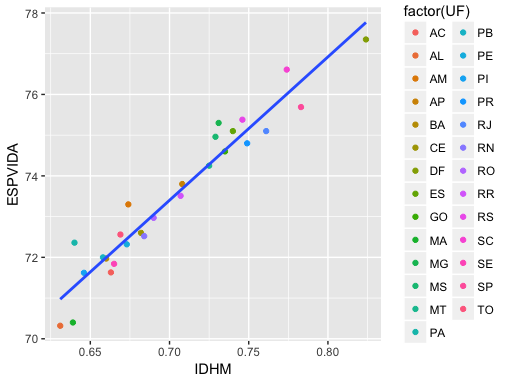
\includegraphics[scale=0.3]{LM-IDHMxESPVIDA.png} \quad
% 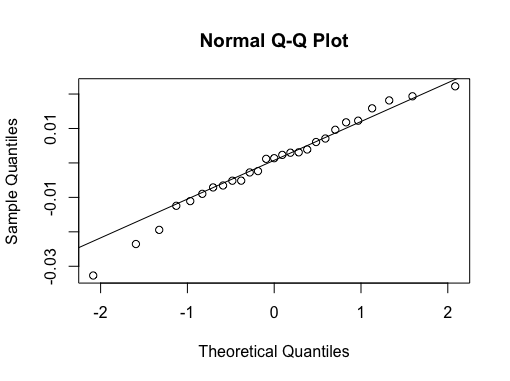
\includegraphics[scale=0.3]{QQNORM-IDHMxESPVIDA.png}}
% \caption{Relação linear IDHM x Esperança de Vida.}
% \label{LM-IDHMxESPVIDA}
% \end{figure}

% Na figura: \ref{LM-IDHMxESPVIDA} observamos a distribuição que mais se ajustou a reta e que obteve maior índice de correlação com IDHM conforme visto na tabela: \ref{Correlação de Pearson de IDHM}.

% \begin{figure}[H]
% \center
% {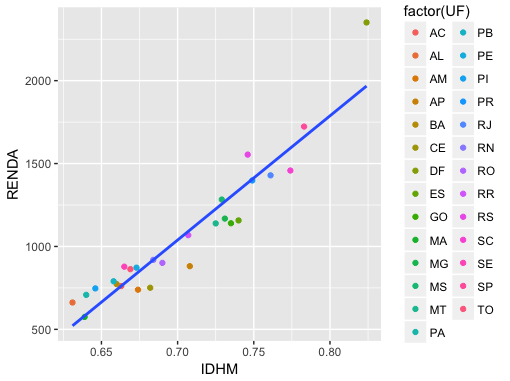
\includegraphics[scale=0.3]{LM-IDHMxRENDA.png} \quad
% 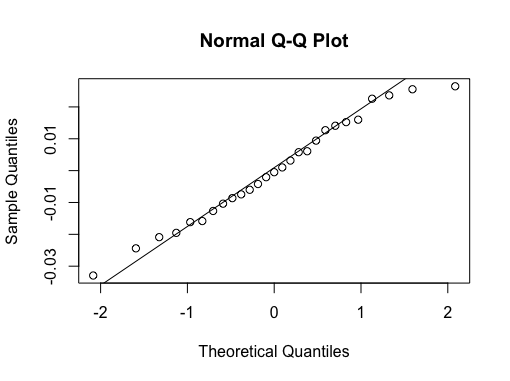
\includegraphics[scale=0.3]{QQNORM-IDHMxRENDA.png}}
% \caption{Relação linear IDHM x RENDA.}
% \label{LM-IDHMxRENDA}
% \end{figure}

% Na Figura: \ref{LM-IDHMxRENDA} identificamos o comportamento linear da distribuição assim como nos resíduos, ajustado a reta, um comportamento esperado visto que a renda é uma variável pertencente ao cálculo do IDHM.

\begin{figure}[H]
\center
{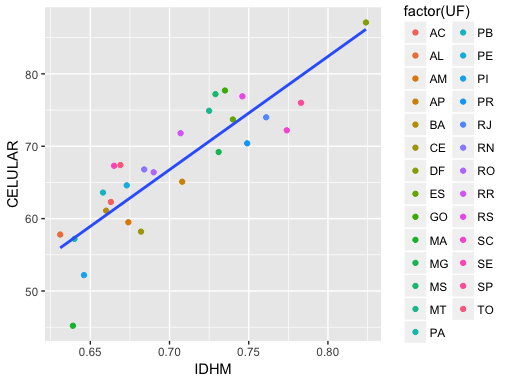
\includegraphics[scale=0.3]{./figuras/LM-IDHMxCELULAR.png} \quad
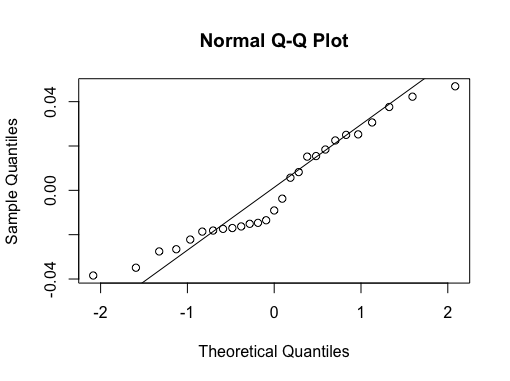
\includegraphics[scale=0.3]{./figuras/QQNORM-IDHMxCELULAR.png}}
\caption{Relação linear IDHM x Posse de celular.}
\label{LM-IDHMxCELULAR}
\end{figure}

Na figura: \ref{LM-IDHMxCELULAR} constatamos que a distribuição é linear, possue uma dispersão mais elevada que as outras variáveis e consequentemente maior resíduos, contudo ainda tem uma correlação significativa conforme resultados verificados na tabela: \ref{Correlação de Pearson de IDHM}, por este motivo foi uma surpresa verificar que esta variável também possue correlação com IDHM.

\begin{figure}[H]
\center
{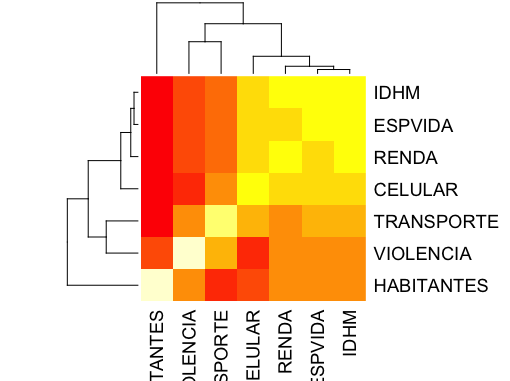
\includegraphics[scale=0.5]{./figuras/COR-Tabela.png}}
\caption{Correlação entre as variáveis.}
\label{COR-Tabela}
\end{figure}

Na figura: \ref{COR-Tabela} observamos o \emph{Heat Map}, mapa de calor, nele verificamos as relações entre as variáveis, onde as cores mais intensas como o Amarelo que identificam as variáveis com maior correlação, e as menos intensas como vermelho possuem menos correlação.

\begin{table}[H]
\centering
\caption{Regreção Linear RENDA + CELULAR + ESPVIDA}
\label{Regreção Linear RENDA + CELULAR + ESPVIDA}
\begin{tabular}{@{}lllll@{}}
\toprule
\multicolumn{5}{c}{\textbf{LM - IDHM $\sim$ RENDA + CELULAR + ESPVIDA}}                                          \\ \midrule
\multicolumn{5}{c}{\textbf{Resíduos}}                                                                            \\
\textbf{Min}         & \textbf{1Q}       & \textbf{Median}     & \textbf{3Q}      & \textbf{Max}                 \\
-0.0252268           & -0.0074518        & 0.0006573           & 0.0068847        & 0.0138412                    \\
\multicolumn{5}{c}{\textit{\textbf{Coeficiêntes}}}                                                               \\
\textit{\textbf{}}   & \textbf{Estimado} & \textbf{Std. Error} & \textbf{t value} & \textbf{Pr(\textgreater|t|)} \\
\textbf{(Intercept)} & -5.359e-01        & 1.705e-01           & -3.142           & 0.004564 **                  \\
\textbf{RENDA}       & 5.017e-05         & 1.193e-05           & 4.207            & 0.000336 ***                 \\
\textbf{CELULAR}     & 1.745e-04         & 4.506e-04           & 0.387            & 0.702021                     \\
\textbf{ESPVIDA}     & 1.597e-02         & 2.564e-03           & 6.229            & 2.35e-06 ***                 \\
\multicolumn{5}{l}{Signif. codes:     0 ‘***’ 0.001 ‘**’ 0.01 ‘*’ 0.05 ‘.’ 0.1 ‘ ’ 1}                            \\
\multicolumn{5}{l}{Residual standard error: 0.009889 on 23 degrees of freedom}                                   \\
\multicolumn{5}{l}{Multiple R-squared: 0.9654      Adjusted R-squared: 0.9609}                                   \\
\multicolumn{5}{l}{F-statistic: 214.1 on 3 and 23 DF      p-value: \textless 2.2e-16}                            \\ \bottomrule
\end{tabular}
\end{table}

Na tabela: \ref{Regreção Linear RENDA + CELULAR + ESPVIDA} verificamos os dados de uma regressão linear multivariada, construída com os dados das variáveis que mais se destacaram no estudo, e testamos para identificar qual a influência de cada variável quando são testadas em conjunto.

% Discussão: Quais conclusões tirou? Como isso mudou a fronteira do conhecimento?
\section{Discussão}

Tendo o Índice de Desenvolvimento Humano Municipal (IDHM) como uma variável dependente para mensurar a qualidade de vida da população dos estados brasileiros, entre as seis variáveis escolhidas para como explicativas para IDHM, três se mostraram estatisticamente significativas a 5\%: Esperança de Vida obteve R$^2$=0.9312, indica que cerca de 93\% da variação de IDHM é explicada por Esperança de Vida e obteve uma correlação alta de 0.9649 cerca de 96\%, já Renda obteve R$^2$=0.8939, indica cerca de 89\% de variação do IDHM e obteve correlação 0.9454 cerca de 94\% e Celular que obteve R$^2$=07553 cerca de 75\% da variação de IDHM e resultando em uma correlação de 0.8690 cerca de 86\%, todos estes dados vistos nas tabelas: \ref{tabela_estimativas_MQO} e \ref{Correlação de Pearson de IDHM}.
As demais variáveis não se destacaram expressivamente, contudo vale salientar que a variável Violência apesar de ter uma correlação negativa: -0.5532 em nossa pequena amostra, ainda assim entendemos que necessitaremos maiores estudos para definir se esta variável realmente não implica em queda do IDHM ou se é apenas uma variável que pode contribuir mas não influenciar diretamente no IDHM, pois observamos em alguns estudos\cite{Ferreira2015}\cite{Cruz2016}\cite{Luciana2007}\cite{loureiroimpacto} constatamos que a violência diminui a qualidade de vida da população. Nesta amostra esta variável não demonstrou grande influência no IDHM.

Quando as três variáveis: Esperança de Vida, Renda e Celular são testadas em uma regressão multivariada conforme dados expostos na tabela: \ref{Regreção Linear RENDA + CELULAR + ESPVIDA}, Esperança de Vida e Renda descrevem com R$^2$=96\% de variação de IDHM, a variável Celular, apesar de no teste multivariado não atingir índices esperados para explicar IDHM na regressão multivariada, pode contribuir em conjunto com outras variáveis socioeconômicas que não foram aqui estudadas.

De acordo com os dados expostos constatamos que um acréscimo de 0.5 à 1\% nas variáveis explicativas de qualidade de vida da população dos estados brasileiros, podem levar a um aumento no IDHM, o que nos leva a uma reflexão sobre a qualidade de vida atual do povo brasileiro, onde grande parte da população dos municípios apenas detém o mínimo para atender suas necessidades básicas, levando-nos assim a afirmar que qualquer melhoria certamente levará a um aumento considerável na qualidade de vida desta população.

\ifCLASSOPTIONcaptionsoff
  \newpage
\fi

\bibliographystyle{IEEEtran}
\bibliography{./bibtex/bib/referencias}
\end{document}